%!TeX root=../pridetop.tex
\chapter[Chapter \thechapter]{}
	
\begin{figure}[t!]
\centering
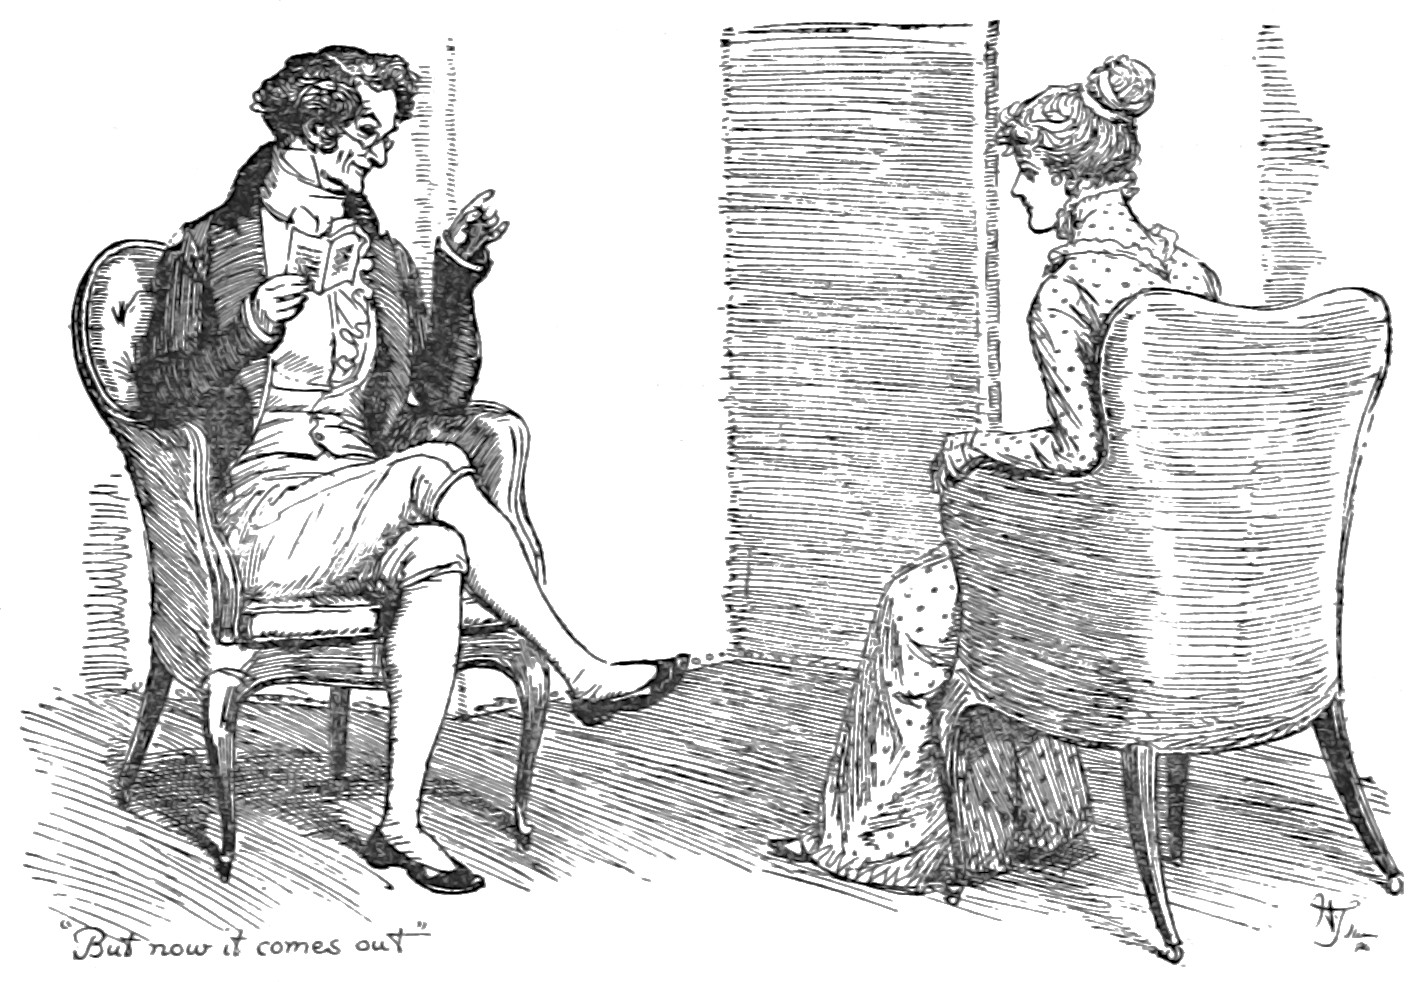
\includegraphics[width=\linewidth]{57top}
\captionlistentry{»But now it comes out«}
\end{figure}


\lettrine[lines=6,image=true]{initials/chap57t}{he}  discomposure of spirits which this extraordinary visit threw Elizabeth into could not be easily overcome; nor could she for many hours learn to think of it less than incessantly. Lady Catherine, it appeared, had actually taken the trouble of this journey from Rosings for the sole purpose of breaking off her supposed engagement with Mr Darcy. It was a rational scheme, to be sure! but from what the report of their engagement could originate, Elizabeth was at a loss to imagine; till she recollected that \textit{his} being the intimate friend of Bingley, and \textit{her} being the sister of Jane, was enough, at a time when the expectation of one wedding made everybody eager for another, to supply the idea. She had not herself forgotten to feel that the marriage of her sister must bring them more frequently together. And her neighbours at Lucas Lodge, therefore, (for through their communication with the Collinses, the report, she concluded, had reached Lady Catherine,) had only set \textit{that} down as almost certain and immediate which \textit{she} had looked forward to as possible at some future time.

In revolving Lady Catherine's expressions, however, she could not help feeling some uneasiness as to the possible consequence of her persisting in this interference. From what she had said of her resolution to prevent the marriage, it occurred to Elizabeth that she must meditate an application to her nephew; and how he might take a similar representation of the evils attached to a connection with her she dared not pronounce. She knew not the exact degree of his affection for his aunt, or his dependence on her judgment, but it was natural to suppose that he thought much higher of her Ladyship than \textit{she} could do; and it was certain, that in enumerating the miseries of a marriage with \textit{one} whose immediate connections were so unequal to his own, his aunt would address him on his weakest side. With his notions of dignity, he would probably feel that the arguments, which to Elizabeth had appeared weak and ridiculous, contained much good sense and solid reasoning.

If he had been wavering before, as to what he should do, which had often seemed likely, the advice and entreaty of so near a relation might settle every doubt, and determine him at once to be as happy as dignity unblemished could make him. In that case he would return no more. Lady Catherine might see him in her way through town; and his engagement to Bingley of coming again to Netherfield must give way.

»If, therefore, an excuse for not keeping his promise should come to his friend within a few days,« she added, »I shall know how to understand it. I shall then give over every expectation, every wish of his constancy. If he is satisfied with only regretting me, when he might have obtained my affections and hand, I shall soon cease to regret him at all.«

The surprise of the rest of the family, on hearing who their visitor had been, was very great: but they obligingly satisfied it with the same kind of supposition which had appeased Mrs Bennet's curiosity; and Elizabeth was spared from much teasing on the subject.

The next morning, as she was going down stairs, she was met by her father, who came out of his library with a letter in his hand.

»Lizzy,« said he, »I was going to look for you: come into my room.«

She followed him thither; and her curiosity to know what he had to tell her was heightened by the supposition of its being in some manner connected with the letter he held. It suddenly struck her that it might be from Lady Catherine, and she anticipated with dismay all the consequent explanations.

She followed her father to the fireplace, and they both sat down. He then said,—

»I have received a letter this morning that has astonished me exceedingly. As it principally concerns yourself, you ought to know its contents. I did not know before that I had \textit{two} daughters on the brink of matrimony. Let me congratulate you on a very important conquest.«

The colour now rushed into Elizabeth's cheeks in the instantaneous conviction of its being a letter from the nephew, instead of the aunt; and she was undetermined whether most to be pleased that he explained himself at all, or offended that his letter was not rather addressed to herself, when her father continued,—

»You look conscious. Young ladies have great penetration in such matters as these; but I think I may defy even your sagacity to discover the name of \textit{your} admirer. This letter is from Mr Collins.«

»From Mr Collins! and what can \textit{he} have to say?«

»Something very much to the purpose, of course. He begins with congratulations on the approaching nuptials of my eldest daughter, of which, it seems, he has been told by some of the good-natured, gossiping Lucases. I shall not sport with your impatience by reading what he says on that point. What relates to yourself is as follows:—»Having thus offered you the sincere congratulations of Mrs Collins and myself on this happy event, let me now add a short hint on the subject of another, of which we have been advertised by the same authority. Your daughter Elizabeth, it is presumed, will not long bear the name of Bennet, after her eldest sister has resigned it; and the chosen partner of her fate may be reasonably looked up to as one of the most illustrious personages in this land.« Can you possibly guess, Lizzy, who is meant by this? »This young gentleman is blessed, in a peculiar way, with everything the heart of mortal can most desire,—splendid property, noble kindred, and extensive patronage. Yet, in spite of all these temptations, let me warn my cousin Elizabeth, and yourself, of what evils you may incur by a precipitate closure with this gentleman's proposals, which, of course, you will be inclined to take immediate advantage of.« Have you any idea, Lizzy, who this gentleman is? But now it comes out. »My motive for cautioning you is as follows:—We have reason to imagine that his aunt, Lady Catherine de Bourgh, does not look on the match with a friendly eye.« \textit{Mr Darcy}, you see, is the man! Now, Lizzy, I think I have surprised you. Could he, or the Lucases, have pitched on any man, within the circle of our acquaintance, whose name would have given the lie more effectually to what they related? Mr Darcy, who never looks at any woman but to see a blemish, and who probably never looked at \textit{you} in his life! It is admirable!«

Elizabeth tried to join in her father's pleasantry, but could only force one most reluctant smile. Never had his wit been directed in a manner so little agreeable to her.

»Are you not diverted?«

»Oh, yes. Pray read on.«

»»After mentioning the likelihood of this marriage to her Ladyship last night, she immediately, with her usual condescension, expressed what she felt on the occasion; when it became apparent, that, on the score of some family objections on the part of my cousin, she would never give her consent to what she termed so disgraceful a match. I thought it my duty to give the speediest intelligence of this to my cousin, that she and her noble admirer may be aware of what they are about, and not run hastily into a marriage which has not been properly sanctioned.« Mr Collins, moreover, adds, »I am truly rejoiced that my cousin Lydia's sad business has been so well hushed up, and am only concerned that their living together before the marriage took place should be so generally known. I must not, however, neglect the duties of my station, or refrain from declaring my amazement, at hearing that you received the young couple into your house as soon as they were married. It was an encouragement of vice; and had I been the rector of Longbourn, I should very strenuously have opposed it. You ought certainly to forgive them as a Christian, but never to admit them in your sight, or allow their names to be mentioned in your hearing.« \textit{That} is his notion of Christian forgiveness! The rest of his letter is only about his dear Charlotte's situation, and his expectation of a young olive-branch. But, Lizzy, you look as if you did not enjoy it. You are not going to be \textit{missish}, I hope, and pretend to be affronted at an idle report. For what do we live, but to make sport for our neighbours, and laugh at them in our turn?«

»Oh,« cried Elizabeth, »I am exceedingly diverted. But it is so strange!«

»Yes, \textit{that} is what makes it amusing. Had they fixed on any other man it would have been nothing; but \textit{his} perfect indifference and \textit{your} pointed dislike make it so delightfully absurd! Much as I abominate writing, I would not give up Mr Collins's correspondence for any consideration. Nay, when I read a letter of his, I cannot help giving him the preference even over Wickham, much as I value the impudence and hypocrisy of my son-in-law. And pray, Lizzy, what said Lady Catherine about this report? Did she call to refuse her consent?«

To this question his daughter replied only with a laugh; and as it had been asked without the least suspicion, she was not distressed by his repeating it. Elizabeth had never been more at a loss to make her feelings appear what they were not. It was necessary to laugh when she would rather have cried. Her father had most cruelly mortified her by what he said of Mr Darcy's indifference; and she could do nothing but wonder at such a want of penetration, or fear that, perhaps, instead of his seeing too \textit{little}, she might have fancied too \textit{much}.